\documentclass{article}
\usepackage[utf8]{inputenc}
\usepackage[spanish]{babel}
\usepackage{graphicx, wrapfig, subcaption, setspace, booktabs}


\usepackage{imakeidx} %indice

\usepackage{amsmath,amssymb}
\usepackage[export]{adjustbox}
\usepackage{url, lipsum}
\usepackage{tgbonum}
\usepackage{hyperref}
\usepackage{xcolor}
\spanishdecimal{.} %Evita que posteriormente latex cambien el punto por coma
%\usepackage{subfigure}

\usepackage{tikz,tkz-tab}%Permite hacer cajas o algo así
\usetikzlibrary{matrix,arrows, positioning,shadows,shadings,backgrounds,calc, shapes, tikzmark}
\usepackage{tcolorbox, empheq}% Permite darle color a las cajas
\tcbuselibrary{skins,breakable,listings,theorems}

\DeclareUnicodeCharacter{2212}{-}
\usepackage{float}
\usepackage{multicol}

%\usepackage{pgfplots}



\makeindex %indice

\begin{document}\label{principal}

\title{Material de métodos numéricos}
\author{Fernando Vazquez Valdez}
%\date{ Hoy merengues }



\maketitle


\begin{abstract} %Resumen
\centering
Temario de métodos numéricos.
\end{abstract}
\newpage

\begin{center}
\section*{1. Introducción a los métodos numéricos}
\end{center}

\input{2. Errores de redondeo y aritmética computacional}
\section*{Algoritmos y convergencia} 

A lo largo del texto examinaremos procedimientos de aproximación, llamados algoritmos, involucrando secuencias de cálculos. Un \textbf{algoritmo} es un proceso que describe, de manera precisa, una secuencia finita de pasos a realizar en un orden en específico. El objetivo del algoritmo es implementar un procedimiento para resolver un problema o aproximar una solución del mismo.

Nosotros usamos un \textbf{pseudocódigo} para describir el algoritmo. Este pseudocódigo especifica la forma de la entrada a suministrar y la forma de la salida deseada.

\begin{tcolorbox}[colback=blue!15!]
\subsubsection*{Ilustración}
El siguiente algotirmo calcula $x_1+x_2+\cdot\cdot\cdot+ x_N=\displaystyle\sum_{i=1}^{N} x_i$ dando \textit{N} y los números $x_1+x_2+\cdot\cdot\cdot x_N$.
\\ \\
ENTRADA $N,x_1+x_2+\cdot\cdot\cdot x_N$

SALIDA $SUM=\sum_{i=1}^{N} x_i$.

PASO 1 Asigna $SUM=0$

PASO 2 Para $i=1,2,...,N$ haz

\ \ \ \ \ \ \ \ \ \ \ \ \ \ \ \ \ \ Asigna $SUM=SUM+x_i$ (Suma el siguiente término)

PASO 3 Salida (SUM);

\ \ \ \ \ \ \ \ \ \ \ \ ALTO.
\end{tcolorbox}
\newpage

\begin{center}
\section*{2. Solución a ecuaciones en una variable}
\end{center}

\section*{2.1 Método de bisección}

En esta sección consideraremos uno de los problemas más básicos del aproximación numérica, el \textbf{problema de encontrar una raíz}. Este proceso involucra encontrar una \textbf{raíz}, o solución, a una ecuación de la forma $f(x)=0$, para la función dada $f$. Una raíz de dicha ecuación también es llamada un \textbf{cero} de la función $f$.
\\

La primera técnica basada en el \textit{Teorema de valor intermedio}, es llamada \textbf{método de bisección} o \textbf{método de búsqueda binaria}.

Suponga $f$ una función continua definida en el intervalo $[a,b]$, con $f(a)$ y $f(b)$ de signos contrarios. El Teorema de valor intermedio implica la existencia de un número $p$ en $(a,b)$ tal que $f(p)=0$. Aunque el procedimiento funcionará si hay más de una raíz en el intervalo $(a,b)$, asumiremos que la raíz en este intervalo es única. El método requiere una repetida partición por la mitad (o bisección) de subintervalos de $[a,b]$, y, en cada paso, localizar la mitad que contiene a $p$.

\ Sea $a_1=a$, $b_1=b$ y dejemos que $p_1$ sea el punto medio de $[a,b]$; entonces

\begin{equation*}
    p_1=a_1+\frac{b_1-a_1}{2}=\frac{a_1+b_1}{2},
\end{equation*}

\begin{itemize}
    \item Si $f(p_1)=0$, entonces $p=p_1$ y hemos acabado.
    \item Si $f(p_1)\neq0$, entonces $f(p_1)$ tiene el mismo signo que $f(a_1)$ o $f(b_1)$.
    \begin{itemize}
        \item  Si $f(p_1)$ y $f(a_1)$ tienen el mismo signo, $p\in(p_1,b_1)$. Sea $a_2=p_1$ y $b_2=b_1$
        \item  Si $f(p_1)$ y $f(a_1)$ tienen signo opuesto, $p\in(a_1,p_1)$. Sea $a_2=a_1$ y $b_2=p_1$
    \end{itemize}
\end{itemize}

Entonces aplicar de nuevo el proceso al intervalo $[a_2,b_2]$. Esto produce el método descrito en el siguiente algoritmo con su respectiva representación geométrica.

\begin{tcolorbox}[colback=blue!15!]
\subsubsection*{Bisección}
Para encontrar la solución a $f(x)=0$ dada una función continua en el intervalo $[a,b]$, donde $f(a)$ y $f(b)$ tienen el signo opuesto:
\\ \\
ENTRADA Puntos límites $a$, $b$; tolerancia \textit{TOL}; número máximo de iteraciones $N_0$.

SALIDA La solución aproximada \textit{p} o mensaje de falla.

PASO 1 Asigna i=1;

\ \ \ \ \ \ \ \ \ \ \ \ \ \ \ \ \ \ \ \ \ \ $FA=f(a)$

PASO 2 Mientras $i\leq N_0$ ejecuta los pasos 3-6.

\ \ \ \  PASO 3 Asigna $p=a+(b-a)/2$; (calcula $p_i$)

\ \ \ \ \ \ \ \ \ \ \ \ \ \ \ \ \ \ \ \ \ \ \ \ \ $FP=f(p)$
    
\ \ \ \   PASO 4 Si $FP=0$ o $(b-a)/2<TOL$ entonces

\ \ \ \ \ \ \ \ \ \ \ \ \ \ \ \ \ \ SALIDA (p); (proceso completado exitosamente)

\ \ \ \ \ \ \ \ \ \ \ \ \ \ \ \ \ \ ALTO.

\ \ \ \   PASO 5 Asigna $i=i+1$
    
\ \ \ \   PASO 6 Si $FA\cdot FP>0$ entonces asigna $a=p$; (calcula $a_i,b_i$)

\ \ \ \ \ \ \ \ \ \ \ \ \ \ \ \ \ \ \ \ \ \ \ \ \ \ \ \ \ \ \ \ \ \ \ \ \ \ \ \ \ \ \ \ \ \ \ \ \ \ \ \ \ \ \ $FA=FP$

\ \ \ \ \ \ \ \ \ \ \ \ \ \ \ \ \ \ \ \ \ \ \ De otro modo asigna $b=p$ (FA no sufre cambios)

PASO 7 SALIDA ('El método falló después de $N_0$ iteraciones $N_0=$',$N_0$);

\ \ \ \ \ \ \ \ \ \ \ \ \ (El proceso fue exitoso.)

\ \ \ \ \ \ \ \ \ \ \ \ \ ALTO.


\end{tcolorbox}

\begin{figure*}[!h]
 \begin{center}
    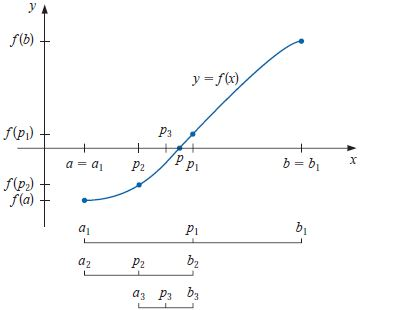
\includegraphics[width=0.8\textwidth]{Biseccion.JPG}
    %\caption{Rapidez de corte vs esfuerzo cortante MAB}
 \end{center}
\end{figure*} 

\subsubsection*{Ejemplo}
Muestra que $f(x)=x^3+4x^2-10=0$ tiene una raíz en $[1,2]$, y usa el método de bisección para determinar una aproximación a la raíz que tenga una precisión de al menos $10^{-4}$.

\textbf{Solución}. Dado que $f(1)=-5$ y $f(2)=14$ el teorema de valor intermedio asegura que ésta función, al ser continua, tiene una raíz en $[1,2]$.

Para la primera iteración del método de bisección usamos el punto medio de $[1,2]$ y obtenemos $f(1.5)=2.375>0$. Eso nos indica que debemos seleccionar el intervalo $[1,1.5]$ para la segunda iteración. Ahora encontramos que $f(1.25)=-796875>0$ entonces nuestro nuevo intervalo es $[1.25,1.5]$ con punto medio en $1.375$. Continuando de esta manera obtenemos la \ref{tab:tabla2}:

\begin{table}[h!]
\centering
    \begin{tabular}{||c c c c c||}
    \hline 
    \hline
        n & $a_n$ & $b_n$ & $p_n$ & $f(p_n)$ \\
    \hline 
    \hline 
        1 & 1.0 & 2.0 & 1.5 & 2.375 \\
        2 & 1.0 & 1.5 & 1.25 & -1.79687 \\
        3 & 1.25 & 1.5 & 1.375 & 0.16211 \\
        4 & 1.25 & 1.375 & 1.3125 & −0.84839 \\
        5 & 1.3125 & 1.375 & 1.34375 & −0.35098 \\
        6 & 1.34375 & 1.375 & 1.359375 & −0.09641 \\
        7 & 1.359375 & 1.375 & 1.3671875 & 0.03236 \\
        8 & 1.359375 & 1.3671875 & 1.36328125 & −0.03215 \\
        9 & 1.36328125 & 1.3671875 & 1.365234375 & 0.000072 \\
        10 & 1.36328125 & 1.365234375 & 1.364257813 & −0.01605 \\
        11 & 1.364257813 & 1.365234375 & 1.364746094 & −0.00799 \\
        12 & 1.364746094 & 1.365234375 & 1.364990235 & −0.00396 \\
        13 & 1.364990235 & 1.365234375 & 1.365112305 & −0.00194 \\
        \hline
        \hline 
    \end{tabular}
    \caption{Bisección}
    \label{tab:tabla2}
\end{table}



Como observación final, para determinar que subintervalo $[a_n.b_n]$ contiene la raíz de $f$, es mejor hacer uso de la función \textbf{signo}, que es definida como:

\begin{equation*}
    sgn(x)= \left\{ \begin{array}{lcc}
             -1 &   si  & x < 0 \\
             \\ 0 &  si &  x = 0 \\
             \\ 1 &  si  & x > 0
             \end{array}
   \right.
\end{equation*}

Dado que la prueba

\begin{equation*}
    sgn(f(a_n))sgn(f(p_n))<0 \ \ \ \ en \ vez \ de \  f(a_n)f(p_n)<0
\end{equation*}

da el mismo resultado pero evita la posibilidad de saturación o sub-desbordamiento en la multiplicación de $f(a_n)$ con $f(p_n)$
\newpage

\section*{2.2 Método punto fijo o sustitución sucesiva}

Un punto fijo para una función es un número en el que el valor de la función no cambia cuando se aplica la función.
\\

\begin{tcolorbox}[colback=gray!5!]
\subsubsection*{Definición}
El número \textit{p} es un \textbf{punto fijo} de una función dada $g$ si $g(p)=p$.
\end{tcolorbox}

En esta sección consideraremos el problema de encontrar soluciones mediante punto fijo y su conexión con los problemas de encontrar raíces. Ambos son de similares en el siguiente sentido:

\begin{itemize}
    \item Dado el problema de encontrar la raíz de $f(p)=0$, podemos definir las funciones $g$  con un punto fijo en $p$ de varias formas, por ejemplo: 
    \begin{center}
        $g(x)=x-f(x)$ o como $g(x)=x +3f(x)$.
    \end{center}
    \item Por el contrario si la función $g$ tiene un punto fijo en $p$, entonces la función definida por 
    \begin{equation*}
        f(x)=x-g(x)
    \end{equation*}
    tiene un cero en $p$.
\end{itemize}

Aunque los problemas que deseamos están en la forma de búsqueda de raíces, la forma de punto fijo es más fácil de analizar, y ciertas elecciones de punto fijo conducen a una técnicas de búsqueda de raíz poderosas.

\subsubsection*{Ejemplo}
Determine cualquier punto fijo de la función $g(x)=x^2-2$.

\textbf{Solución}. Un punto fijo de g tiene la propiedad de 
\begin{center}
    $p=g(p)=p^2-2$ lo cual implica que $0=p^2-p-2=(p+1)(p-2)$.
\end{center}

Un punto fijo de $g$ ocurre precisamente cuando la gráfica de $y=g(x)$ corta en $y=x$, entonces $g$ tiene dos puntos fijos, uno en $p=-1$ y otro en $p=2$ como se muestra. \ref{tab:fig}

\begin{figure*}[h!]
\centering
  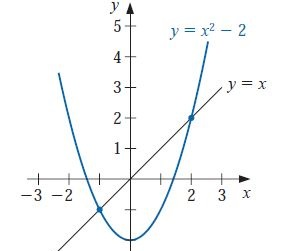
\includegraphics[width=0.6\textwidth]{Puntofijo.JPG}
\caption{Punto fijo}
\label{tab:fig}
\end{figure*} 


Por otra parte, cuando no podamos determinar el punto fijo de alguna función porque no podamos resolver para $p$ dicha ecuación se considerarán aproximaciones con precisión determinada. A continuación se muestra como hacerlo.

Para aproximar el punto dijo de una función $g$ elegimos una aproximación inicial $p_0$ y generamos la secuencia $\left\lbrace p_n\right\rbrace ^\infty_{n=0}$ siendo $p_n=g(p_{n-1})$, para cada $n>1$. Si la secuencia converge a $p$ y $g$ es continua, entonces

\begin{equation*}
    p = \lim_{n \to \infty}(p_n)=\lim_{n \to \infty}g(p_{n-1})=g\left(\lim_{n \to \infty}(p_{n-1})\right)=g(p),
\end{equation*}

Y se obtiene una solución a $x=g(x)$. Esta técnica es llamada \textbf{punto fijo}. El procedimiento se ilustra en \ref{tab:fig2}:

\begin{figure*}[h!]
\centering
  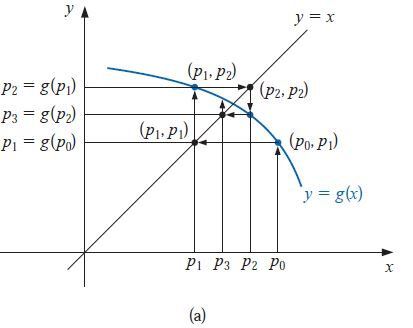
\includegraphics[width=0.6\textwidth]{Puntofijo2.JPG}
\caption{Punto fijo 2}
\label{tab:fig2}
\end{figure*} 

\begin{tcolorbox}[colback=blue!15!]
\subsubsection*{Punto fijo}
Para encontrar la solución a $p=g(p)$ dada la aproximación inicial $p_0$:
\\ \\
ENTRADA aproximación inicial $p_0$; tolerancia \textit{TOL}; número máximo de iteraciones $N_0$.

SALIDA La solución aproximada \textit{p} o mensaje de falla.

PASO 1 Asigna i=1;

PASO 2 Mientras $i\leq N_0$ ejecuta los pasos 3-6.

\ \ \ \  PASO 3 Asigna $p=g(p_0)$; (calcula $p_i$)

\ \ \ \  PASO 4 Si $|p-p_0|<TOL$ entonces

\ \ \ \ \ \ \ \ \ \ \ \ \ \ \ \ \ \ SALIDA (p); (proceso completado exitosamente)

\ \ \ \ \ \ \ \ \ \ \ \ \ \ \ \ \ \ ALTO.

\ \ \ \   PASO 5 Asigna $i=i+1$
    
\ \ \ \   PASO 6 Asigna $p_0=p$; (Actualiza $p_0$.)

PASO 7 SALIDA ('El método fallo después de $N_0$ iteraciones $N_0=$',$N_0$);

\ \ \ \ \ \ \ \ \ \ \ \ \ (El proceso fue exitoso.)

\ \ \ \ \ \ \ \ \ \ \ \ \ ALTO.


\end{tcolorbox}

A continuación se ilustran algunas características de la iteración funcional.

\subsubsection*{Ejemplo}
La ecuación $x^3+4x^2-10=0$ tiene una única raíz en $[1,2]$. Hay muchas formas de cambiar la ecuación para la forma de punto fijo $x=g(x)$ utilizando simple manipulación algebraica. Por ejemplo, para obtener la función $g$ descrita en el inciso (c) se manipula la ecuación $x^3+4x^2-10=0$ como a continuación:

\begin{center}
$4x^2=10-x^3$, entonces $x^2=\frac{1}{4}(10-x^3)$ y $x=\pm\frac{1}{2}(10-x^3)^{1/2}$
\end{center}

\begin{tcolorbox}[colback=gray!5!]
\subsubsection*{Nota}
Es importante resaltar que no todas las formas llevan a convergencia aunque todas son soluciones de la ecuación original, por ejemplo:
\end{tcolorbox}

\quad\quad\quad \textbf{(a)} $x=g_1(x)=x-x^3-4x^2+10$
\quad\quad\quad \textbf{(b)} $x=g_2(x)=(\frac{10}{x}-4x)^{1/2}$

\quad\quad\quad \textbf{(c)} $x=g_3(x)=\frac{1}{2}(10-x^3)^{1/2}$
\quad\quad\quad \textbf{(d)} $x=g_4(x)=(\frac{10}{x+4})^{1/2}$

\quad\quad\quad \textbf{(e)} $x=g_5(x)=x-\frac{x^3+4x^2-10}{3x^2+8x}$
\\
\\

Con $p_0=1.5$ se obtiene la tabla \ref{tab:tabla4}:

\begin{table}[h!]
\centering
    \begin{tabular}{||c c c c c c||}
    \hline 
    \hline
        n & (a) & (b) & (c) & (d) & (e) \\
    \hline 
    \hline 
        0 & 1.5 & 1.5 & 1.5 & 1.5 & 1.5 \\
        1 & −0.875 & 0.8165 & 1.286953768 & 1.348399725 &  1.373333333 \\
        2 & 6.732 & 2.9969 & 1.402540804 & 1.367376372 & 1.365262015 \\
        3 & −469.7 & $−8.65^{1/2}$ & 1.345458374 & 1.364957015 &  1.365230014 \\
        4 & $1.03\times10^{8}$ &  & 1.375170253 & 1.365264748 &  1.365230013 \\
        5 &  &  & 1.360094193 & 1.365225594 & \\
        6 &  &  & 1.367846968 & 1.365230576 & \\
        7 &  &  & 1.363887004 & 1.365229942 & \\
        8 &  &  & 1.365916734 & 1.365230022 & \\
        9 &  &  & 1.364878217 & 1.365230012 & \\
        10 &  &  & 1.365410062 & 1.365230014 & \\
        15 &  &  & 1.365223680 & 1.365230013 & \\
        20 &  &  & 1.365230236 &  & \\
        25 &  &  & 1.365230006 &  & \\
        30 &  &  & 1.365230013 &  & \\
        \hline
        \hline 
    \end{tabular}
    \caption{Punto fijo}
    \label{tab:tabla4}
\end{table}


La raíz real es 1.365230013. Comparando el resultados del algoritmo de bisección dado en ese ejemplo, se puede ver que los resultados excelentes se han obtenido para las opciones (c), (d) y (e) (el método de bisección requiere 27 iteraciones para esta precisión). Es interesante notar que la elección (a) fue divergente y que (b) se convirtió en indefinido porque involucra la raíz cuadrada de un número negativo. 
\newpage

\input{6. Método de Newton y sus variantes}
\newpage

\section*{2.4 Falsa posición}

Cada par sucesivo de aproximaciones en el método de Bisección incluye una raíz $p$ de la ecuación; esto es, por cada entero positivo $n$ hay una raíz entre $a_n$ y $b_n$. Esto implica que por cada $n$ la iteración del método de Bisección satisface:

\begin{center}
    $|p_n-p|<\frac{1}{2}|a_n-b_n|$,
\end{center}

Lo cual provee una frontera del error fácilmente calculada por las aproximaciones.
La frontera de la raíz no está garantizada para ninguno de los métodos de Newton.

El método de \textbf{Falsa posición} genera aproximaciones e incluye una prueba que asegura que la raíz está delimitada mediante iteraciones sucesivas. 

Primero se elijen las aproximaciones iniciales $p_0$ y $p_1$ con $f(p_0)\cdot f(p_1)<0$ la aproximación $p_2$ es elegida como la intersección de la linea generada de unir $(p_0,f(p_0))$ y $(p_1,f(p_1))$ con el eje x. Para decidir que recta secante usar para calcular $p_3$ se considera $f(p_2)\cdot f(p_1)<0$ o más correctamente $sgnf(p_2)\cdot sgnf(p_1)$.

\begin{itemize}
    \item Si $sgnf(p_2)\cdot sgnf(p_1)<0$ entonces $p_1$ y $p_2$ delimitan a una raíz. Se elige $p_3$ como la intersección de la linea generada de unir $(p_1,f(p_1))$ y $(p_2,f(p_2))$ con el eje x.
    \item Si no, se elige $p_3$ como la intersección de la linea generada de unir $(p_0,f(p_0))$ y $(p_2,f(p_2))$ con el eje x y luego se intercambian los índices en $p_0$ y $p_1$.
\end{itemize}

De manera similar, una vez encontrado $p_3$ el signo de $f(p_3)\cdot f(p_2)$ determina si se usa $p_2$ y $p_3$ o $p_3$ y $p_1$ para calcular $p_4$. En último caso se realiza el reetiquetado de $p_2$ y $p_1$. El reetiquetado asegura que la raíz se encuentra dentro de la frontera mediante iteraciones sucesivas. El proceso es descrito por el algoritmo de \textbf{falsa posición} y la figura \ref{tab:fig5}.

\begin{figure*}[h!]
\centering
  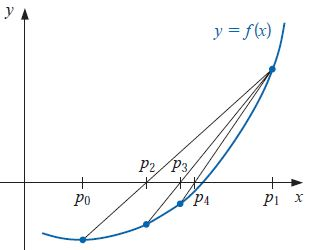
\includegraphics[width=0.6\textwidth]{Falsaposicion.JPG}
\caption{Falsa posición}
\label{tab:fig5}
\end{figure*} 

\begin{tcolorbox}[colback=blue!15!]
\subsubsection*{Falsa posición}
Para encontrar la solución a $f(x)=0$ dada la función continua $f$ en el intervalo $[p_0,p_1]$ donde $f(p_0)$ y $f(p_1)$ tienen signos opuestos:
\\ \\
ENTRADA aproximaciones iniciales $p_0$, $p1$; tolerancia \textit{TOL}; número máximo de iteraciones $N_0$.

SALIDA La solución aproximada \textit{p} o mensaje de falla.

PASO 1 Asigna i=2;

\ \ \ \ \ \ \ \ \ \ \ \ \ \ \ \ \ \ \ \ \ \ \ \ $q_0=f(p_0)$;

\ \ \ \ \ \ \ \ \ \ \ \ \ \ \ \ \ \ \ \ \ \ \ \ $q_1=f(p_1)$.

PASO 2 Mientras $i\leq N_0$ ejecuta los pasos 3-7.

\ \ \ \  PASO 3 Asigna $p=p_1 -q_1(p_1-p_0)/(q_1-q_0) $; (calcula $p_i$)

\ \ \ \  PASO 4 Si $|p-p_0|<TOL$ entonces

\ \ \ \ \ \ \ \ \ \ \ \ \ \ \ \ \ \ SALIDA (p); (proceso completado exitosamente)

\ \ \ \ \ \ \ \ \ \ \ \ \ \ \ \ \ \ ALTO.

\ \ \ \   PASO 5 Asigna $i=i+1$;

\ \ \ \ \ \ \ \ \ \ \ \ \ \ \ \ \ \ \ \ \ \ \ \ \ \ \ \ $q=f(p)$.
    
\ \ \ \   PASO 6 Si $q\cdot q_1<0$ entonces asigna $p_0=p_1$; 

\ \ \ \ \ \ \ \ \ \ \ \ \ \ \ \ \ \ \ \ \ \ \ \ \ \ \ \ \ \ \ \ \ \ \ \ \ \ \ \ \ \ \ \ \ \ \ \ \ \ \ \ \ \ \ \ \ \ \ $q_0=q_1$.

\ \ \ \   PASO 7 Asigna $p_1=p$;

\ \ \ \ \ \ \ \ \ \ \ \ \ \ \ \ \ \ \ \ \ \ \ \ \ \ \ \ $q_1=q$.

PASO 8 SALIDA ('El método fallo después de $N_0$ iteraciones $N_0=$',$N_0$);

\ \ \ \ \ \ \ \ \ \ \ \ \ (El proceso fue exitoso.)

\ \ \ \ \ \ \ \ \ \ \ \ \ ALTO.


\end{tcolorbox}

\subsubsection*{Ejemplo}
Use el método de falsa posición para encontrar la solución a $x=cos x$.

\textbf{Solución}. Se usarán las aproximaciones iniciales $p_0=0.5$ y $p_1=\pi/4$. La tabla \ref{tab:tabla6} muestra el resultado de aplicar el método de falsa posición a $f(x)=cosx-x$.

\begin{table}[h!]
\centering
    \begin{tabular}{||c c||}
    \hline 
    \hline
        \multicolumn{2}{c}{\textbf{Falsa posición}}\tabularnewline
        $n$ & $p_n$      \\
    \hline 
    \hline 
        0 & 0.5 \\
        1 & 0.7853981635 \\
        2 & 0.7363841388 \\
        3 & 0.7390581392 \\
        4 & 0.7390848638 \\
        5 & 0.7390851305 \\
        6 & 0.7390851332 \\
        \hline
        \hline 
    \end{tabular}
\caption{Falsa posición cosx-x}
\label{tab:tabla6} 
\end{table}
\newpage

\section*{2.5 Newton varias variables}

En esta sección se utilizará una extensión del método de Newton para aproximar la solución al problema solo que esta vez los conceptos y herramientas del calculo serán en varias variables. Con afán de hacer lo más sencillo posible el cambio de una variable a varias variables se realizarán comparaciones geométricas entre éstas dos. 

\subsection*{Funciones de varias variables}
Primero: pensemos en una función cuya representación geométrica es una parábola figura \ref{tab:funcion}


\begin{figure*}[h!]
\centering
  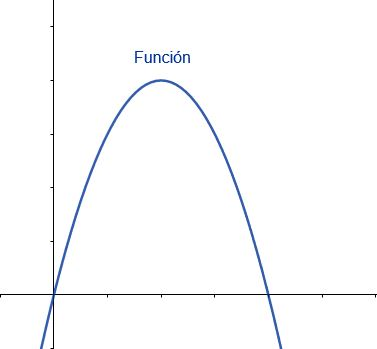
\includegraphics[width=0.4\textwidth]{funcion1.JPG}
\caption{Parábola}
\label{tab:funcion}
\end{figure*} 

Ahora pensemos que rotamos la parábola en torno a la linea que se forma de unir el vértice con el foco, esto provocará que la gráfica deje de estar en el plano y ahora se convierta en un objeto conocido como paraboloide: figura \ref{tab:fun3}.

\begin{figure*}[h!]
\centering
  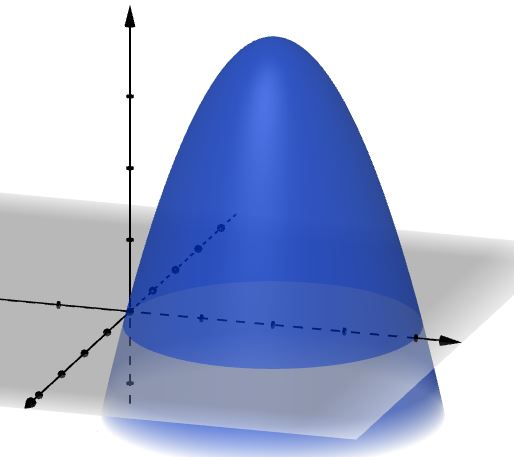
\includegraphics[width=0.45\textwidth]{funcion2.JPG}
\caption{Paraboloide}
\label{tab:fun3}
\end{figure*} 

Pues bien, como se podrá intuir, las funciones de varias variables $f(x,y,z,...)$ son la generalización de las funciones de una variable $f(x)$ con las cuales estamos más familiarizados, esto quiere decir que ahora ya no solo dependerá de una variable sino de dos o más y que, dependiendo del plano con el cual ``toquemos'' a la función de varias variables nos dará distintas funciones (proyecciones) en dicho plano.

\subsection*{Derivada en varias variables}
Ahora recordemos que la representación geométrica de la derivada es la \textbf{recta tangente} de la función $f(x)=y$, en otras palabras, es la recta que interseca a la función en un solo punto y si la evaluamos nos indica cual es el valor de la pendiente en dicho punto. 

En las figuras \ref{tab:fig6}, \ref{tab:fig7} y \ref{tab:fig8} se ilustra como es que la recta se va ``moviendo'' por la gráfica hasta solo tocar en un punto donde es la recta de interés. 

\begin{multicols}{3}
\begin{figure}[H]
\centering
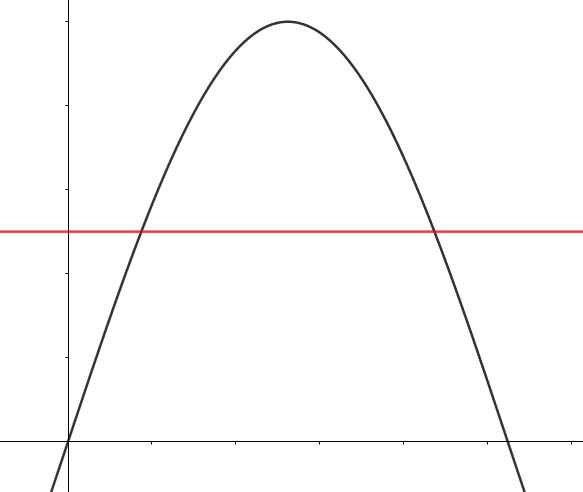
\includegraphics [ width =0.3\textwidth ]{aprox1.jpg}
\caption{Cuerda}
\label{tab:fig6}
\end{figure}
\begin{figure}[H]
\centering
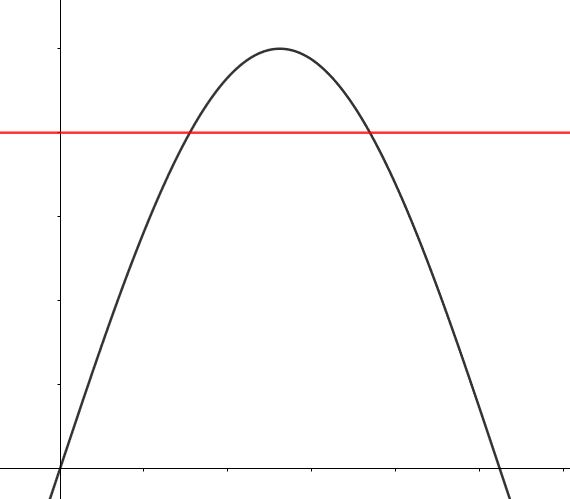
\includegraphics [ width =0.3\textwidth ]{aprox2.JPG}
\caption{Secante}
\label{tab:fig7}
\end{figure}
\begin{figure}[H]
\centering
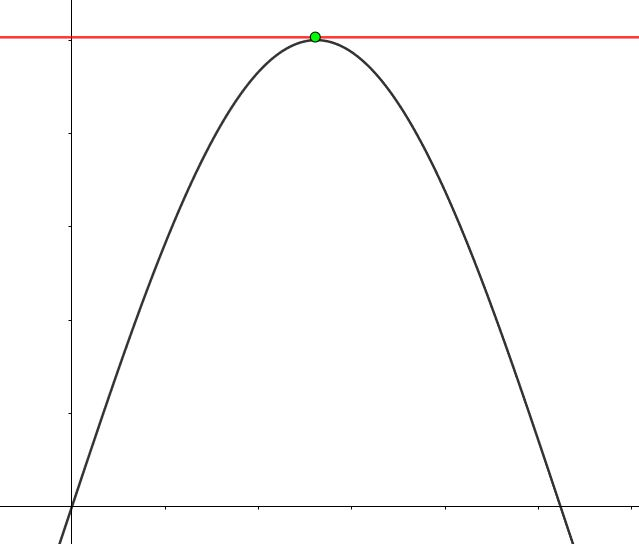
\includegraphics [ width =0.3\textwidth ]{aprox3.JPG}
\caption{\textbf{Tangente}}
\label{tab:fig8}
\end{figure}
\end{multicols}

Es de esperarse que en funciones de varias variables se pueda derivar con respecto a las variables que aparecen en la función y no solo una como anteriormente se hacía; por ejemplo si tenemos la función $f(x,y,z)=(f_1,f_2,f_3)=(2x^2yz,5xy^4z,3xyz^3)$ podremos \textbf{derivar parcialmente} con respecto a $x$, $y$ o $z$ entonces tendremos:

\begin{equation*}
    \frac{\partial}{\partial x} f(x,y,z)=\frac{\partial}{\partial x}(f_1,f_2,f_3)=(\frac{\partial}{\partial x} f_1,\frac{\partial}{\partial x} f_2,\frac{\partial}{\partial x} f_3)=(\frac{\partial}{\partial x} 2x^2yz,\frac{\partial}{\partial x} 5xy^4z,\frac{\partial}{\partial x} 3xyz^3)
\end{equation*}
Notemos que la derivada es respecto a $x$ por lo tanto todas las demás variables son constantes ante ésta y por ello ``salen'' de la derivada y queda:

\begin{equation*}
\begin{split}
    \frac{\partial}{\partial x} f(x,y,z)&=(2yz \frac{\partial}{\partial x}x^2,5y^4z\frac{\partial}{\partial x}x,3yz^3\frac{\partial}{\partial x}x)\\
    &=(2yz(2x),5y^4z(1),3yz^3(1))
\end{split}
\end{equation*}
Finalmente
\begin{equation*}
    \frac{\partial}{\partial x} f(x,y,z)=(4xyz,5y^4z,3yz^3)
\end{equation*}

Análogamente con las otras dos derivadas parciales pero ahora con $y$ y $z$:

\begin{equation*}
\begin{split}
    \frac{\partial}{\partial y} f(x,y,z)&=(2x^2z \frac{\partial}{\partial y}y,5xz\frac{\partial}{\partial y}y^4,3xz^3\frac{\partial}{\partial y}y)\\
    &=(2x^2z(1),5xz(4y^3),3xz^3(1))\\
    &=(2x^2z,20xy^3z,3xz^3)
\end{split}
\end{equation*}

Y

\begin{equation*}
\begin{split}
    \frac{\partial}{\partial z} f(x,y,z)&=(2x^2y \frac{\partial}{\partial z}z,5xy^4\frac{\partial}{\partial z}z,3xy\frac{\partial}{\partial z}z^3)\\
    &=(2x^2y(1),5xy^4(1),3xy(3z^2))\\
    &=(2x^2y,5xy^4,9xyz^2)
\end{split}
\end{equation*}

Entonces tenemos los siguientes resultados:

\begin{equation*}
\begin{split}
    (\frac{\partial}{\partial x} f_1,\frac{\partial}{\partial x} f_2,\frac{\partial}{\partial x} f_3)&=(4xyz,5y^4z,3yz^3)\\
    (\frac{\partial}{\partial y} f_1,\frac{\partial}{\partial y} f_2,\frac{\partial}{\partial y} f_3)&=(2x^2z,20xy^3z,3xz^3)\\ 
    (\frac{\partial}{\partial z} f_1,\frac{\partial}{\partial z} f_2,\frac{\partial}{\partial z} f_3)&=(2x^2y,5xy^4,9xyz^2)
\end{split}
\end{equation*}

Que si lo escribimos de manera matricial es:

\begin{equation*}
\Large
\begin{pmatrix}
\frac{\partial f_1}{\partial x} & \frac{\partial f_2}{\partial x} & \frac{\partial f_3}{\partial x}\\
\frac{\partial f_1}{\partial y} & \frac{\partial f_2}{\partial y} & \frac{\partial f_3}{\partial y}\\
\frac{\partial f_1}{\partial z} & \frac{\partial f_2}{\partial z} & \frac{\partial f_3}{\partial z}
\end{pmatrix}
=
\begin{pmatrix}
4xyz & 5y^4z & 3yz^3\\
2x^2z & 20xy^3z & 3xz^3\\
2x^2y & 5xy^4 & 9xyz^2
\end{pmatrix}
\end{equation*} 

Pues bien, si transponemos la matriz (los vectores columna cambian a vectores fila o viceversa) queda de la forma:

\begin{equation*}
\Large
\begin{pmatrix}
\frac{\partial f_1}{\partial x} & \frac{\partial f_1}{\partial y} & \frac{\partial f_1}{\partial z}\\
\frac{\partial f_2}{\partial x} & \frac{\partial f_2}{\partial y} & \frac{\partial f_2}{\partial z}\\
\frac{\partial f_3}{\partial x} & \frac{\partial f_3}{\partial y} & \frac{\partial f_3}{\partial z}
\end{pmatrix}
=
\begin{pmatrix}
4xyz & 2x^2z & 2x^2y\\
5y^4z & 20xy^3z & 5xy^4\\
3yz^3 & 3xz^3 & 9xyz^2
\end{pmatrix}
\end{equation*} 

Y lo que acabamos de obtener se le conoce como \textbf{la matriz jacobiana} que será de suma importancia en el tema que nos compete.

Cabe resaltar que se puede dar el caso de tener una función general con $m$ componentes $(f_1,f_2,\dotso,f_m)$ y dependiente de $n$ variables $f(x_1,x_2,\dotso,x_n)$, en dicho caso la matriz jacobiana es no necesariamente cuadrada y se escribe de la forma:

\begin{equation*}
\Large
\textbf{Matriz \ jacobiana \ general}\Rightarrow 
\begin{pmatrix}
\frac{\partial f_1}{\partial x_1} & \dotsb & \frac{\partial f_1}{\partial x_n}\\
\vdots & \ddots & \vdots\\
\frac{\partial f_m}{\partial x_1} & \dotsb & \frac{\partial f_m}{\partial x_n}
\end{pmatrix}
\end{equation*} 


\subsection*{Método de Newton en varias variables}
Ahora bien, retomemos la ecuación del método de Newton para una variable:

\begin{equation*}
    p_n= p_{n-1} -\frac{f(p_{n-1})}{f'(p_{n-1})}, \ para \ n\geq 1.
\end{equation*}

Primero hay que notar que la función depende una sola variable $p_{n-1}$ y también el punto de partida guarda información sólo de la variable $x$ puesto que $p_0=x_0$; ahora bien, el propósito de todo lo anterior fue dar las bases para la generalización del método y es muy natural pensar que, al tener una \textbf{función de varias variables} todos los demás elementos sean también en varias variables como se muestra en la tabla \ref{tab:tabla7}.

\begin{table}[h!]
\centering
    \begin{tabular}{||c c c||}
    \hline 
    \hline
        \multicolumn{3}{c}{\textbf{Generalización}}\tabularnewline
        Una variable &  & Varias variables (dependiente de $x,y$) \\
    \hline 
    \hline 
        $f(p_{n-1})$ & $\rightarrow$ & \textbf{Función} \\
        $f'(p_{n-1})$ & $\rightarrow$ & $\textbf{Jacobiano de f}$ \\
        $p_n$  & $\rightarrow$ & \textbf{Vector $p_n$} \\
        $p_{n-1}$ & $\rightarrow$ & \textbf{Vector $p_{n-1}$} \\
        \hline
        \hline 
    \end{tabular}
\caption{Una variable - varias variables}
\label{tab:tabla7} 
\end{table}

Nota: en la literatura al \textbf{jacobiano de f} se puede encontrar como \textbf{$J_f$}, D\textbf{f} o $ \nabla\textbf{f} $. 

Entonces la ecuación para el método de Newton en varias variables es:

\begin{equation*}
    \textbf{p}_n= \textbf{p}_{n-1} -[\nabla\textbf{f}(p_{n-1})]^{-1} \textbf{f}(p_{n-1}), \ para \ n\geq 1.
\end{equation*}

Cuyo proceso es descrito por el algoritmo de \textbf{Newton en varias variables}

\begin{tcolorbox}[colback=blue!15!]
\subsubsection*{Newton en varias variables}
Para encontrar la solución a $\textbf{f}(x,y)=0$ dada la aproximación inicial $\textbf{p}_0$:
\\ \\
ENTRADA aproximación inicial $p_0$; tolerancia \textit{TOL}; número máximo de iteraciones $N_0$.

SALIDA La solución aproximada \textit{p} o mensaje de falla.

PASO 1 Asigna i=1;

PASO 2 Mientras $i\leq N_0$ ejecuta los pasos 3-6.

\ \ \ \  PASO 3 Asigna $\textbf{p}=\textbf{p}_0 -[\nabla\textbf{f}(\textbf{p}_0)]^{-1} \textbf{f}(\textbf{p}_0) $; (calcula $p_i$)

\ \ \ \  PASO 4 Si $||\textbf{p}-\textbf{p}_0||<TOL$ entonces

\ \ \ \ \ \ \ \ \ \ \ \ \ \ \ \ \ \ SALIDA (p); (proceso completado exitosamente)

\ \ \ \ \ \ \ \ \ \ \ \ \ \ \ \ \ \ ALTO.

\ \ \ \   PASO 5 Asigna $i=i+1$
    
\ \ \ \   PASO 6 Asigna $\textbf{p}_0=\textbf{p}$; (Actualiza $p_0$.)

PASO 7 SALIDA ('El método fallo después de $N_0$ iteraciones $N_0=$',$N_0$);

\ \ \ \ \ \ \ \ \ \ \ \ \ (El proceso fue exitoso.)

\ \ \ \ \ \ \ \ \ \ \ \ \ ALTO.


\end{tcolorbox}
\newpage

\section*{4. Ecuaciones diferenciales ordinarias}

El movimiento de un péndulo que se balancea asumiendo ciertas simplificaciones es descrito por una ecuación diferencial de segundo orden:

\begin{equation*}
    \frac{d^2\theta}{d t^2} +\frac{g}{L}sin\theta=0.
\end{equation*}

Donde L es el ángulo del péndulo, $g\approx9.81 m/s^2$ es la constante gravitacional de la tierra y $\theta$ es el ángulo que el péndulo hace con la vertical. Además, se especifica que el movimiento inicia en  $\theta(t_0)=\theta_0$ y su velocidad en dicho punto es $\theta'(t_0)=\theta'_0$; estas especificaciones se llaman \textbf{condiciones iniciales} y el problema se conoce como \textbf{problema con condiciones iniciales o valores iniciales}. Para valores pequeños de $\theta$ la aproximación $\theta\approx sin\theta$ puede ser utilizada para simplificar el problema a un problema lineal con condiciones iniciales:

\begin{equation*}
    \frac{d^2\theta}{d t^2} +\frac{g}{L}\theta=0, \ \ \theta(t_0)=\theta_0, \ \ \theta'(t_0)=\theta'_0.
\end{equation*}

Este problema ahora puede ser resuelto con las técnicas tradicionales de ecuaciones diferenciales.

\subsection*{4.1 Método de Euler}

El método de Euler es la técnica de aproximación más sencilla para resolver los problemas con condiciones iniciales. El objetivo del método de Euler es obtener aproximaciones al problema con valores iniciales.

\begin{equation*}
    \frac{dy}{dt}=f(t,y), \ \ a\leq t\leq b, \ \ y(a)=\alpha.
\end{equation*}

Sin embargo, este método no obtendrá una aproximación a $y(t)$ sino una aproximación a $y$ en varios valores -llamados \textbf{puntos malla}- en el intervalo $[a,b]$ y una vez encontrada la solución aproximada en dichos puntos las siguientes soluciones aproximadas de los otros puntos serán calculadas mediante interpolación.

Primero se realiza la estipulación de que los puntos malla están uniformemente distribuidos en el intervalo $[a,b]$. Esta condición se asegura eligiendo un número entero positivo N y seleccionando los puntos de malla de la siguiente manera:

\begin{equation*}
    t_i=a+ih, \ \ \ \ con \ \ i=0,1,2, \dotsc, N.
\end{equation*}

La distancia $h$ es comúnmente llamada \textbf{tamaño de paso} y se calcula mediante $h=(b-a)/N=t_{i+1}-t_i$. 

Ahora se usará el teorema de Taylor para derivar el método de Euler. Suponga que $y(t)$, la única solución a la ecuación $\frac{dy}{dt}=f(t,y)$, tiene dos derivadas continuas es el intervalo $[a,b]$ entonces para cada $i=0,1,2, \dotsc, N$, 

\begin{equation*}
    y(t_{i+1})=y(t_i)+(t_{i+1}-t_i)+\frac{(t_{i+1}-t_i)^2}{2}y''(\xi_i),
\end{equation*}

para un número $\xi_i$ en $(t_i,t_{i+1})$. Pero como $h=t_{i+1}-t_i$ se obtiene: 

\begin{equation*}
    y(t_{i+1})=y(t_i)+h y'(t_i)+\frac{h^2}{2}y''(\xi_i),
\end{equation*}

pero como $y(t)$ satisface la ecuación diferencial original,

\begin{equation*}
    y(t_{i+1})=y(t_i)+h f(t_i,y(t_i))+\frac{h^2}{2}y''(\xi_i).
\end{equation*}

El método de Euler considera $wi\approx y(t_i)$ para cada $i=0,1,2, \dotsc, N$, por eliminación del término restante. Así, el método de Euler es: 

\begin{equation*}
\begin{split}
    w_0&=\alpha \\
    w_{i+1}&=w_i+hf(t_i,w_i), \ \ para \ cada \ i=0,1,2, \dotsc, N-1.
\end{split}
\end{equation*}

\subsubsection*{Ejemplo}

Utilice el método de Euler para aproximar la solución a

\begin{equation*}
    y'=y-t^2+1, \ \ 0\leq t\leq 2, \ \ y(0)=0.5.
\end{equation*}

en $t=2$. Simplemente se ilustrará los pasos de la técnica cuando se tiene $h=0.5$. 

Para este problema $f(t,y)=y-t^2+1$, entonces

\begin{equation*}
\begin{split}
    w_0&=y(0)=0.5; \\
    w_1&=w_0+0.5(w_0-(0.0)^2+1)=0.5+0.5(1.5)=1.25; \\
    w_2&=w_1+0.5(w_1-(0.5)^2+1)=1.25+0.5(2.0)=2.25; \\
    w_3&=w_2+0.5(w_2-(1.0)^2+1)=2.25+0.5(2.25)=3.375;
\end{split}
\end{equation*}

Entonces

\begin{equation*}
    y(2)\approx w_4=w_3+0.5(w_3-(1.5)^2+1)=3.375+0.5(2.125)=4.4375.
\end{equation*}


\begin{tcolorbox}[colback=blue!15!]
\subsubsection*{Método de Euler}
Para aproximar la solución del problema con valores iniciales

\begin{equation*}
    y'=f(t,y), \ \  a\leq t\leq b, \ \ y(a)=\alpha,
\end{equation*}

en un intervalo [a,b] dividido en (N+1) del mismo tamaño:
\\ \\
ENTRADA Puntos extremos a,b; entero N; condición inicial $\alpha$.

SALIDA Aproximación $w$ a $y$ en $(N+1)$ valores de $t$.
\\ \\
PASO 1 Asigna h=(b-a)/N;

\ \ \ \ \ \ \ \ t=a;

\ \ \ \ \ \ \ \ $w=\alpha$;

\ \ \ \ \  SALIDA (t,w).

PASO 2 Para $i=1,2,\dotsc, N$ ejecuta los pasos 3 y 4.

\ \ \ \  PASO 3 Asigna $w=w+hf(t,w)$; (calcula $w_i$.)

\ \ \ \ \ \ \ \ \ \ \ \ \ \ \ \ \ \ \ \ \ \ \ \ \ \ \ \ \ $t=a+ih$; (calcula $t_i$.)

\ \ \ \  PASO 4  SALIDA (t,w)

PASO 5 Alto.

\end{tcolorbox}

Para interpretar el método de Euler geométricamente es necesario notar que cuando $w_i$ es cercano a la aproximación de $y(t_i)$ la suposición de que el problema está bien planteado implica que:

\begin{equation*}
    f(t_i,w_i)\approx y'(t_i)=f(t_i,y(t_i)).
\end{equation*}

El gráfico de la función resaltando $y(t_i)$ se muestra en la figura \ref{tab:fig9}. En la figura \ref{tab:fig10} aparece un paso del método de Euler y en la figura \ref{tab:fig11} aparece una serie de pasos. 

\begin{figure*}[h!]
\centering
  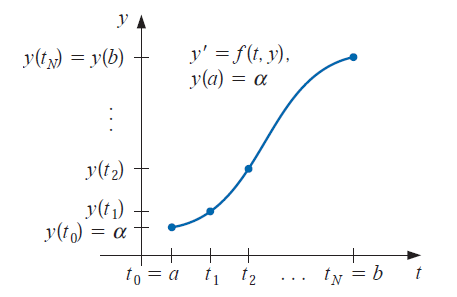
\includegraphics[width=0.65\textwidth]{Euler1.png}
\caption{}
\label{tab:fig9}
\end{figure*} 

\begin{multicols}{2}
\begin{figure}[H]
\centering
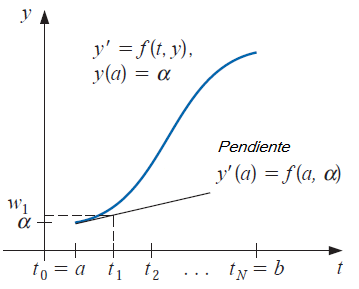
\includegraphics [ width =0.5\textwidth ]{Euler2.png}
\caption{}
\label{tab:fig10}
\end{figure}
\begin{figure}[H]
\centering
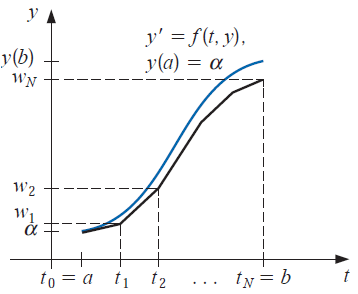
\includegraphics [ width =0.5\textwidth ]{Euler3.png}
\caption{}
\label{tab:fig11}
\end{figure}
\end{multicols}

\subsection*{4.2 Método de Euler mejorado}

Dado que el objeto de las técnicas numéricas es determinar aproximaciones precisas con el mínimo esfuerzo, necesitamos una medida para comparar la eficiencia de varios métodos de aproximación. La primera de ellas que consideramos se denomina \textbf{error de truncamiento local}.

Considere el problema del valor inicial

\begin{equation*}
    y'=f(t,y), \ \  a\leq t\leq b, \ \ y(a)=\alpha, 
\end{equation*}

el método diferencial

\begin{equation*}
\begin{split}
    w_0&=\alpha \\
    w_{i+1}&=w_i+h\Phi(t_i,w_i), \ \ para \ cada \ i=0,1,2, \dotsc, N-1.
\end{split}
\end{equation*}

tiene el \textbf{error de truncamiento local}

\begin{equation*}
    \tau_{i+1}(h)=\frac{y_{i+1}-(y_i+h\Phi(t_i,y_i))}{h}=\frac{y_{i+1}-y_i}{h}-\Phi(t_i,y_i).
\end{equation*}

para cada $i=0,1,2, \dotsc, N-1$ donde $y_i$ y $y_{i+1}$ denotan la solución al tiempo $t_i$ y $t_{i+1}$ respectivamente.
\\

En afán de ir reduciendo cada vez más el error relacionado al método se busca optimizar el proceso de aproximación, ahora bien, para desarrollar un método más preciso que el de Euler se puede modificar éste para mejorarlo, de esta manera surge el \textbf{método de Euler modificado} el cual consta en realizar una corrección intermedia a cada iteración, primero se estima el punto sucesivo y enseguida se hace la corrección de la forma:

\begin{equation*}
    w_{i+1}=w_i+\frac{h}{2}(f(t_i,w_i)+f(t_i+h,w_i+hf(t_i,w_i))).
\end{equation*}

Entonces el algoritmo resultante es:

\begin{equation*}
\begin{split}
    w_0&=\alpha \\
    w^*_{i+1}&=w_i+hf(t_i,w_i), \ \ Estimacion \\
    w_{i+1}&=w_i+\frac{h}{2}(f(t_i,w_i)+f(t_i+h,w^*_{i+1})) \ \ Correccion \\ 
    & \ \ \ \ \ para \ cada \ i=0,1,2, \dotsc, N-1.
\end{split}
\end{equation*}

Y, por lo tanto, el código es el siguiente:


\begin{tcolorbox}[colback=blue!15!]
\subsubsection*{Método de Euler modificado}
Para aproximar la solución del problema con valores iniciales

\begin{equation*}
    y'=f(t,y), \ \  a\leq t\leq b, \ \ y(a)=\alpha,
\end{equation*}

en un intervalo [a,b] dividido en (N+1) del mismo tamaño:
\\ \\
ENTRADA Puntos extremos a,b; entero N; condición inicial $\alpha$.

SALIDA Aproximación $w$ a $y$ en $(N+1)$ valores de $t$.
\\ \\
PASO 1 Asigna h=(b-a)/N;

\ \ \ \ \ \ \ \ t=a;

\ \ \ \ \ \ \ \ $w=\alpha$;

\ \ \ \ \  SALIDA (t,w).

PASO 2 Para $i=1,2,\dotsc, N$ ejecuta los pasos 3 y 5.

\ \ \ \  PASO 3 Asigna $w^*=w+hf(t,w)$; (Estima $w_i$.)

\ \ \ \  PASO 4 Asigna $w=w+\frac{1}{2}h(f(t,w)+f(t+h,w^*))$; (Corrige $w_i$.)

\ \ \ \ \ \ \ \ \ \ \ \ \ \ \ \ \ \ \ \ \ \ \ \ \ \ \ \ \ $t=a+ih$; (calcula $t_i$.)

\ \ \ \  PASO 5  SALIDA (t,w)

PASO 6 Alto.

\end{tcolorbox}

\subsection*{4.3 Método de Runge-Kutta}

Los métodos de Runge-Kutta tienen el error de truncamiento local de alto orden de los métodos de Taylor, pero eliminan la necesidad de calcular y evaluar las derivadas de $f(t, y)$. Antes de presentar las ideas detrás de su derivación, debemos considerar el Teorema de Taylor en dos variables.

\subsubsection*{Teorema de Taylor en dos variables}
Supongamos que $f(t, y)$ y todas sus derivadas parciales de orden menor o igual a $n+1$ son continuas en $D = \{ (t, y) | a\leq t \leq b, c \leq y \leq d \}$, y sea $(t_0, y_0) \in D$. Para todo $(t, y) \in D$, existe $\xi$ entre $t$ y $t_0$ y $\mu$ entre $y$ e $y_0$ con

\begin{equation*}
    f(t,y)=P_n(t,y)+R_n(t,y),
\end{equation*}

donde

\begin{equation*}
\begin{split}
    P_n(t,y)=&f(t_0,y_0)+ \left[ (t-t_0)\frac{\partial f}{\partial t} (t_0,y_0) + (y-y_0)\frac{\partial f}{\partial t} (t_0,y_0) \right] \\ 
    & + \left[ \frac{(t-t_0)^2}{2}\frac{\partial^2 f}{\partial t^2} (t_0,y_0) + (t-t_0)(y-y_0)\frac{\partial^2 f}{\partial t \partial y} (t_0,y_0) + \frac{(y-y_0)^2}{2}\frac{\partial^2 f}{\partial y^2}(t_0,y_0) \right] \\
    & + \dotsi + \left[ \frac{1}{n!} \sum_{j=0}^n \binom{n}{j}(t-t_0)^{n-j}(y-y_0)^j \frac{\partial^n f}{\partial t^{n-j} \partial y^j}(t_0,y_0) \right].
\end{split}
\end{equation*}

Y

\begin{equation*}
    R_n(t,y)=\frac{1}{(n+1)!} \sum_{j=0}^{n+1} \binom{n+1}{j}(t-t_0)^{n+1-j}(y-y_0)^j \frac{\partial^{n+1}f}{\partial t^{n+1-j} \partial y^j}(\xi,\mu).
\end{equation*}

La función $P_n(t, y)$ se llama enésimo polinomio de Taylor en dos variables para la función $f$ sobre $(t_0, y_0)$, y $R_n(t, y)$ es el término restante asociado con $P_n(t, y)$.

\subsubsection*{Método de Runge-Kutta de orden dos}

El primer paso para derivar un método de Runge-Kutta es determinar los valores para $a_1$, $\alpha_1$ y $\beta_1$ con la propiedad de que $a_1 f(t+\alpha_1,y+\beta_1)$ se aproxima:

\begin{equation*}
    T^{(2)}(t,y)=f(t,y)+\frac{h}{2}f'(t,y),
\end{equation*}

con un error no mayor que $O(h^2)$, que es igual al orden del error de truncamiento local para el método de Taylor de orden dos. Ya que

\begin{equation*}
    f'(t,y)=\frac{df}{dt}(t,y)=\frac{\partial f}{\partial t} (t,y) + \frac{\partial f}{\partial y} (t,y)\cdot y'(t) \ \ , \ \ y'(t)= f(t,y)
\end{equation*}

entonces:

\begin{equation*}
    T^{(2)}(t,y)=f(t,y)+\frac{1}{2}\frac{\partial f}{\partial t} (t,y) + \frac{1}{2}\frac{\partial f}{\partial y} (t,y)\cdot f(t,y).
\end{equation*}

Expandiendo 

\begin{equation*}
\begin{split}
       a_1 f(t+\alpha _1, y + \beta _1)=&a_1f(t,y)+a_1\alpha _1 \frac{\partial f}{\partial t} (t,y) + a_1 \beta _1 \frac{\partial f}{\partial y} (t,y) \\
       & + a_1 \cdot R_1(t+\alpha _1, y + \beta _1).
\end{split}
\end{equation*}

Donde

\begin{equation*}
    R_1(t+\alpha _1, y + \beta _1) = \frac{\alpha_1^2}{2} \frac{\partial^2 f}{\partial t^2} (\xi,\mu) + \alpha _1\beta _1 \frac{\partial^2 f}{\partial t \partial y} (\xi,\mu) + \frac{\beta_1^2}{2} \frac{\partial^2 f}{\partial y^2} (\xi,\mu)
\end{equation*}

para algún $/xi$ entre $t$ y $t+\alpha_1$ y $\mu$ entre $ y + \beta _1$.
\\
Igualando los coeficientes de $f$ y sus derivadas se obtiene:

\begin{equation*}
    f(t,y): a_1=1; \ \ \ \ \frac{\partial f}{\partial t} (t,y):a_1 \alpha_1=\frac{h}{2}; \ \ \ \ \frac{\partial f}{\partial y} (t,y):a_1 \beta_1=\frac{h}{2}f(t,y).
\end{equation*}

Por lo tanto los parámetros $a_1$, $\alpha_1$ y $\beta_1$ son:

\begin{equation*}
    a_1=1; \ \ \ \ \alpha_1=\frac{h}{2}; \ \ \ \ \  \beta_1=\frac{h}{2}f(t,y).
\end{equation*}

Entonces

\begin{equation*}
    T^{(2)}(t,y)=f \left(t+ \frac{h}{2},y+\frac{h}{2}f(t,y)\right)-R_1 \left(t+ \frac{h}{2},y+\frac{h}{2}f(t,y)\right)
\end{equation*}

PP 285
\newpage

\section*{5. Sistemas de ecuaciones diferenciales ordinarias}


\newpage

\section*{Apéndice I: Códigos en Matlab}

%\subsection*{Bisección}
\begin{figure*}[h!]
\centering
  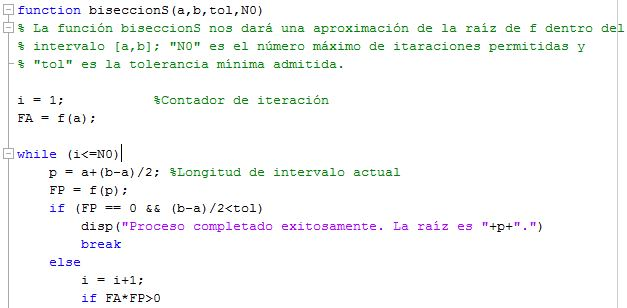
\includegraphics[width=1\textwidth]{BiseccionC1.JPG}
  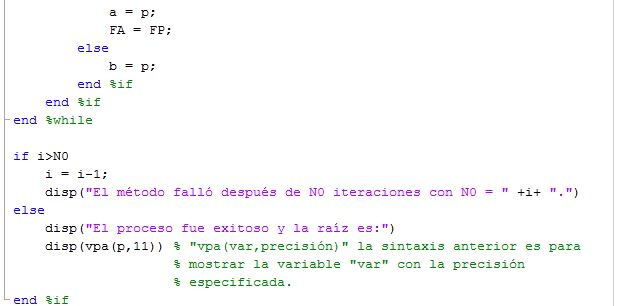
\includegraphics[width=1\textwidth]{BiseccionC2.JPG}
\end{figure*} 

%\subsection*{Falsa posición}
\begin{figure*}[h!]
\centering
  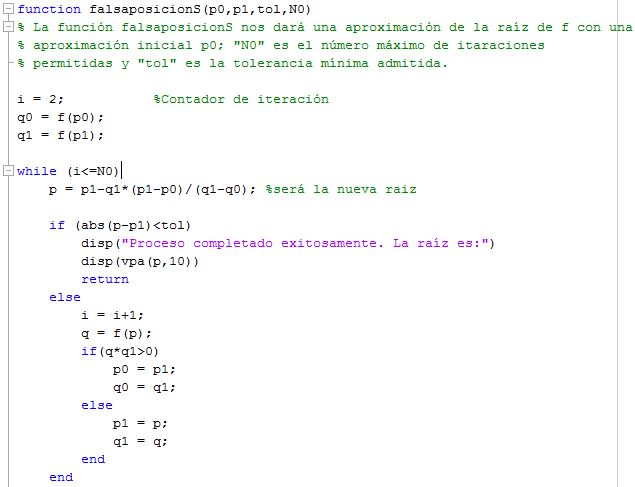
\includegraphics[width=1\textwidth]{FalsaC1.JPG}
  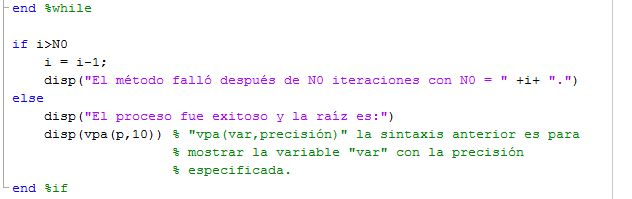
\includegraphics[width=1\textwidth]{FalsaC2.JPG}
\end{figure*} 

%\subsection*{Punto fijo}
\begin{figure*}[h!]
\centering
  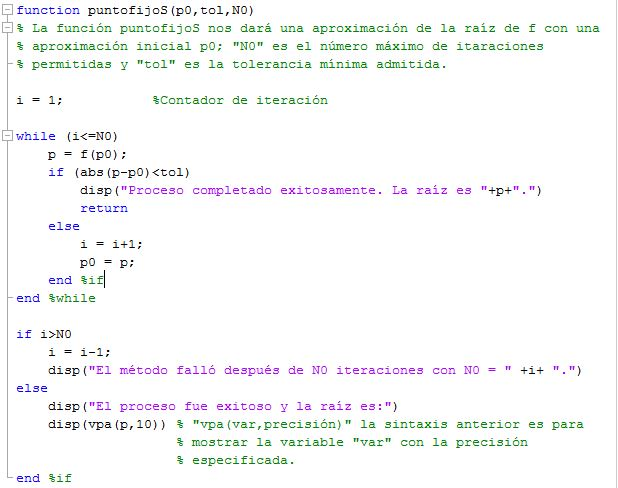
\includegraphics[width=1\textwidth]{PFijoC.JPG}
\end{figure*} 

%\subsection*{Newton}
\begin{figure*}[h!]
\centering
  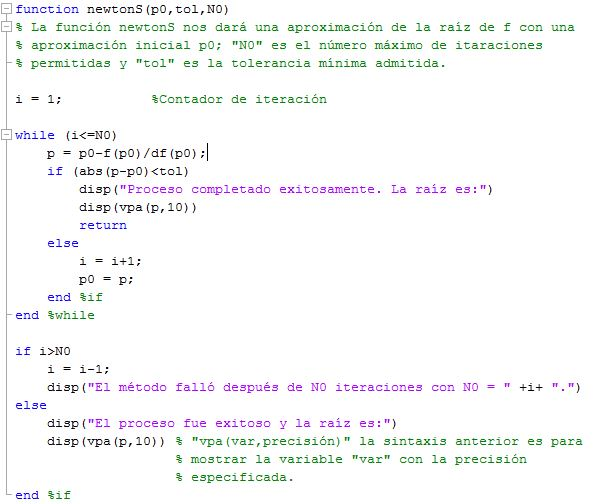
\includegraphics[width=1\textwidth]{NewtonC.JPG}
\end{figure*} 

%\subsection*{Newton en varias variables}
\begin{figure*}[h!]
\centering
  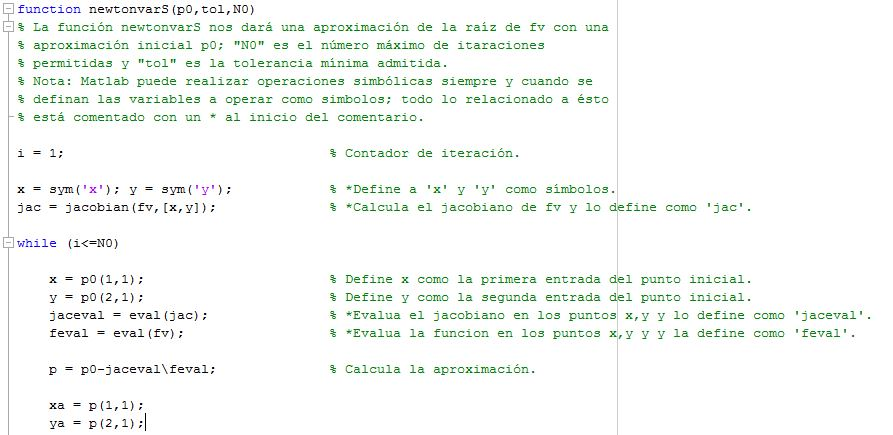
\includegraphics[width=1.2\textwidth]{NewtonVarC1.JPG}
  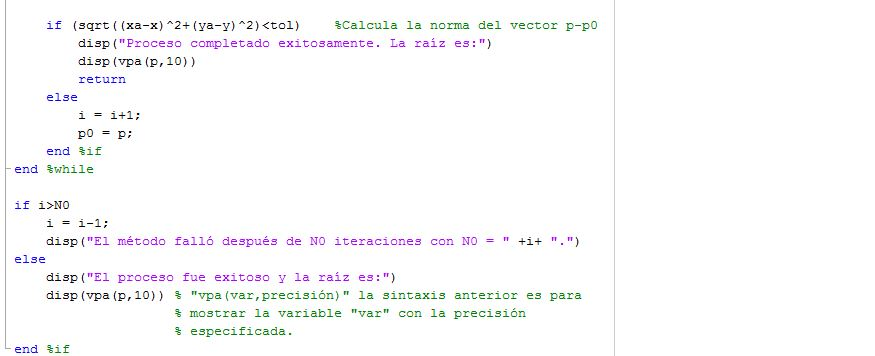
\includegraphics[width=1.2\textwidth]{NewtonVarC2.JPG}
\end{figure*} 

\end{document}
